% CVPR 2025 Paper Template; see https://github.com/cvpr-org/author-kit

\documentclass[10pt,twocolumn,letterpaper]{article}

%%%%%%%%% PAPER TYPE  - PLEASE UPDATE FOR FINAL VERSION
\usepackage{cvpr}              % To produce the CAMERA-READY version
% \usepackage[review]{cvpr}      % To produce the REVIEW version
% \usepackage[pagenumbers]{cvpr} % To force page numbers, e.g. for an arXiv version

% Import additional packages in the preamble file, before hyperref
\input{preamble}

\definecolor{cvprblue}{rgb}{0.21,0.49,0.74}
\usepackage[pagebackref,breaklinks,colorlinks,allcolors=cvprblue]{hyperref}

%%%%%%%%% PAPER ID  - PLEASE UPDATE
\def\paperID{0000} % *** Enter the Paper ID here
\def\confName{CVPR}
\def\confYear{2025}

%%%%%%%%% TITLE
\title{Training-Free Post-Processing for Visual Place Recognition:\\
Replace the Weak Base, Keep the Sequence}

%%%%%%%%% AUTHORS - PLEASE UPDATE
\author{Eunhyeog Jang\\
Seoul National University\\
{\tt\small jang200210@snu.ac.kr}
}

\begin{document}
\maketitle

%%%%%%%%% ABSTRACT
\begin{abstract}
Visual place recognition (VPR) is a core component of robot localization,
providing loop closure and relocalization that bound the drift of metric
odometry. Modern foundation-model descriptors are strong, yet single-frame
retrieval still fails under extreme appearance change and perceptual aliasing.
We study, in a controlled manner, how much \emph{training-free} classical
post-processing can recover on top of \emph{frozen} state-of-the-art VPR
descriptors, adding no learned component. Revisiting SeqSLAM, we observe that
its 2012 weakness was not the sequence idea but its \emph{raw-pixel base}: with
the same sequence step, replacing the base by a stronger classical descriptor
(CLAHE${+}$HOG) lifts Recall@1 from $25.3$ to $96.1$, and a frozen deep
descriptor reaches $98.8$. We then evaluate two classical cues on top of the
frozen descriptor---(A) temporal consistency filtering that exploits the query
being a driving sequence, and (B) geometric verification re-ranking using SIFT
and MAGSAC. On Nordland, temporal filtering lifts Recall@1 by $+33.4$ and
$+12.5$ points for EigenPlaces and SALAD respectively, independent of the
descriptor and robust under a strict $\pm1$-frame ($2.5\,$m) ground-truth
threshold. Geometric re-ranking, in contrast, yields only marginal gains on
strong viewpoint-robust descriptors and can \emph{hurt} when local matching
fails; we propose a simple, learning-free \emph{confidence-adaptive} fusion that
improves all SVOX conditions and, unlike any fixed weight, never regresses.
Finally, a training-free deep${+}$HOG score fusion adds $+11.3$ R@1 at the
single-frame level for the relocalization (no-sequence) regime. The most
valuable training-free signal is the temporal prior; geometry must be applied
adaptively to be safe.
\end{abstract}

%%%%%%%%% BODY
\section{Introduction}
\label{sec:intro}
Localization is fundamental to mobile robotics. Metric odometry and SLAM,
including LiDAR-inertial systems such as FAST-LIO2~\cite{xu2022fastlio2},
estimate a continuous pose but accumulate drift over time. \emph{Visual place
recognition} (VPR) addresses a complementary problem: given a query image,
retrieve which previously seen place it depicts. VPR is the standard mechanism
for \emph{loop closure} and \emph{relocalization}, i.e.\ recognizing revisited
places to correct accumulated drift~\cite{milford2012seqslam}.

This work began from improving LiDAR odometry in geometrically degenerate
environments by re-weighting LiDAR points with visual cues. We found that
re-weighting alone cannot resolve the underlying \emph{observability}
deficiency~\cite{zhang2016degeneracy}, and that obtaining ground truth for a
full multi-sensor system is costly. We therefore kept the same motivation---
robust localization of a driving robot---but moved to camera-based place
recognition, the module that actually corrects odometry drift.

We deliberately add only \emph{non-deep-learning} post-processing on top of a
\emph{frozen} pretrained descriptor, matching the assignment scope. Our
question is: \emph{without any extra training or data, how much can classical
post-processing improve a state-of-the-art descriptor, and which cue helps
which failure mode?} Our contributions are:
\begin{itemize}\itemsep2pt
  \item A \emph{base ladder} that isolates SeqSLAM's real weakness: with the
  sequence step fixed, replacing the raw-pixel base by CLAHE${+}$HOG or a frozen
  deep descriptor determines the ceiling ($+70.8$ and $+35.1$ R@1), and a fully
  classical CLAHE${+}$HOG${+}$sequence pipeline reaches $96.1$ R@1 in real time.
  We cross-check the sequence gain with DTW to show it is not aligner-specific.
  \item A controlled study of two training-free cues---temporal filtering and
  geometric re-ranking---on frozen 2023--2024 descriptors (EigenPlaces,
  SALAD), with the temporal gain shown robust under a strict $\pm1$-frame
  ($2.5\,$m) ground-truth threshold.
  \item An empirical finding that the temporal (sequence) prior is by far the
  most valuable training-free signal ($+12$ to $+33$ R@1), independent of the
  descriptor, whereas geometric verification is marginal on strong descriptors.
  \item A simple, training-free \emph{confidence-adaptive} fusion that, unlike
  any fixed weight, improves every tested condition without regression
  (cf.~\cite{zaffar2024uncertainty}, but using only SIFT inlier counts and
  \emph{no learning}); and a training-free deep${+}$HOG score fusion that adds
  $+11.3$ R@1 at the single-frame level for the no-sequence relocalization case.
\end{itemize}

\section{Related Work}
\label{sec:related}
\noindent\textbf{Global descriptors.} Learned global descriptors dominate VPR,
from NetVLAD~\cite{arandjelovic2016netvlad} to viewpoint-robust
EigenPlaces~\cite{berton2023eigenplaces} and the DINOv2-based
SALAD~\cite{izquierdo2024salad}. We use the latter two, frozen.

\noindent\textbf{Sequence-based VPR.} SeqSLAM~\cite{milford2012seqslam}
post-processes the single-frame similarity matrix using sequence structure;
ConvSequential-SLAM~\cite{tomita2021convsequential} is a training-less
sequence method. Module~A follows this line.

\noindent\textbf{Geometric re-ranking.}
Patch-NetVLAD~\cite{hausler2021patchnetvlad} \emph{trains} patch features for
re-ranking, while a recent model-free re-ranking method~\cite{kanji2024modelfree}
uses \emph{learned} local features. Uncertainty- and query-adaptive re-ranking
has also been studied~\cite{zaffar2024uncertainty}; our adaptive fusion is a
deliberately minimal, learning-free instance of this idea.

\noindent\textbf{Positioning.} We claim no new algorithm for A or B
individually; each is established. Our work differs in that (i) the added
modules are $100\%$ classical (SIFT, Viterbi/SeqSLAM) with \emph{zero} learned
components, (ii) they operate on frozen 2024 foundation descriptors, and
(iii) we isolate the temporal vs.\ geometric cues and propose an adaptive
fusion that fixes the documented failure of naive re-ranking.

\section{Method}
\label{sec:method}
We keep the descriptor frozen and operate on the cosine similarity matrix
$\mathbf{S}\in\mathbb{R}^{T\times N}$ between $T$ queries and $N$ database
images.

\subsection{Module A: Temporal Consistency Filtering}
The query is a driving sequence, so the correct matches lie on a near-diagonal
path of $\mathbf{S}$. We model this with a hidden Markov model: state $x_t$ is
the database index, emission $p(z_t\mid x_t{=}j)\propto\exp(s_{tj}/\tau)$, and
transition restricted to a forward advance $j\in[i+v_{\min}, i+v_{\max}]$ with a
small teleport probability $\epsilon$. We implement three variants:
(i) \textbf{SeqSLAM}---local-contrast normalization then constant-velocity
diagonal window aggregation (offline, bidirectional);
(ii) \textbf{Viterbi}---log-space MAP path
$\delta_t(j)=\max_i[\delta_{t-1}(i)+\log a_{ij}]+\log b_t(j)$;
(iii) \textbf{forward filter}---causal belief propagation (online, real-time).

\subsection{Replace the Weak Base (classical base ladder)}
\label{sec:ladder}
SeqSLAM~\cite{milford2012seqslam} originally fed the sequence step with a
\emph{raw-pixel SAD} base, which collapses under seasonal change. We test the
hypothesis that the weakness was the base, not the sequence idea, by swapping in
stronger \emph{classical} descriptors while keeping the sequence step fixed:
$\text{raw image}\to\text{CLAHE}~\cite{zuiderveld1994clahe}\to
\text{HOG}~\cite{dalal2005hog}\to\text{cosine }\mathbf{S}\to\text{sequence}$.
CLAHE normalizes illumination and HOG encodes gradient structure rather than raw
intensity, so it survives appearance change far better than pixel SAD. We
compare three bases---raw-pixel SAD, CLAHE${+}$HOG (ours), and a frozen deep
descriptor---each single-frame, ${+}$SeqSLAM, and ${+}$DTW. To show the sequence
gain is not specific to one aligner, we also align with standard
\textbf{Dynamic Time Warping}~\cite{sakoe1978dtw} (a monotonic minimum-cost path
on $-\mathbf{S}$, allowing speed variation).

\subsection{Deep${+}$HOG Single-Frame Fusion}
\label{sec:fusion}
For the relocalization regime (no sequence available), we fuse the deep and HOG
\emph{single-frame} scores, $s=a\,\tilde{s}_{\text{deep}}+(1{-}a)\,\tilde{s}_{\text{HOG}}$,
with no learning. The two are complementary---learned semantic invariance vs.\
explicit gradient structure---so the fusion improves single-frame retrieval.

\subsection{Module B: Geometric Re-ranking}
For each query we re-rank the top-$K$ candidates by SIFT correspondences
(ratio test $0.8$) verified with MAGSAC, using the inlier count as a geometric
score. We fuse with the global similarity via
$\text{final}=\alpha\,\widetilde{s}_{\text{glob}}+(1-\alpha)\,\widetilde{n}_{\text{inl}}$,
with per-query min--max normalization $\widetilde{(\cdot)}$.

\subsection{Module B+: Confidence-Adaptive Fusion (ours)}
\label{sec:adaptive}
A fixed $\alpha$ is unsafe: the best value differs per condition, and a low
$\alpha$ that helps clear scenes is catastrophic at night where SIFT fails.
We instead set $\alpha$ \emph{per query} from the geometric evidence. With
$\mathrm{conf}_q=\mathrm{clip}(\max_j n_{qj}/C,\,0,\,1)$ we use
\begin{equation}
\alpha_q = 1-(1-\alpha_{\min})\,\mathrm{conf}_q .
\end{equation}
When inliers are abundant ($\mathrm{conf}_q\!\to\!1$) the fusion trusts
geometry ($\alpha_q\!\to\!\alpha_{\min}$); when matching fails
($\mathrm{conf}_q\!\to\!0$) it falls back to the global order
($\alpha_q\!\to\!1$), which is safe. A single $(\alpha_{\min},C)$ is shared
across all conditions, requiring no per-condition tuning.

\section{Experiments}
\label{sec:exp}
\noindent\textbf{Setup.} Descriptors: EigenPlaces (ResNet50, 2048-d) and SALAD
(DINOv2, 8448-d), both frozen (inference only). Both are trained by their authors
on \emph{city} street-view data (SF-XL, GSV-Cities) and used here zero-shot,
which is why their single-frame retrieval collapses on rural, season-flipped
Nordland. Datasets: \textbf{Nordland}
(winter query vs.\ summer database; a dense, frame-aligned sequence with
extreme seasonal change) for Module~A, and \textbf{SVOX} (Oxford RobotCar,
condition-wise queries) for Module~B. Positives use a $25\,$m UTM threshold
($\approx\pm10$ frames for Nordland). We report Recall@$\{1,5,10\}$.
We excluded St~Lucia (EigenPlaces R@1 $=99.5\%$, a ceiling) and Baidu~Mall
(inconsistent coordinate frames) after empirical checks. Fig.~\ref{fig:heatmap}
shows the Nordland similarity matrix: a bright diagonal (the correct sequence)
amid strong off-diagonal noise, explaining both the single-frame failure and
the headroom for temporal filtering.

\begin{figure}[t]
  \centering
  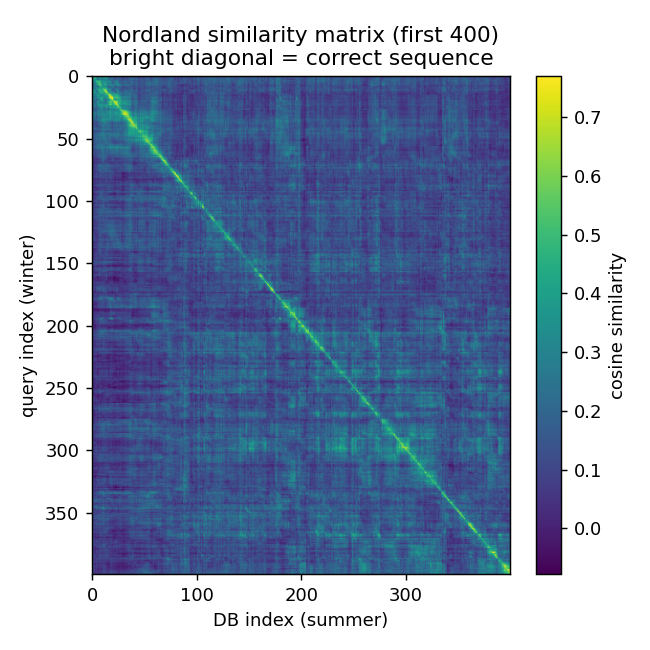
\includegraphics[width=0.82\linewidth]{figures/nordland_heatmap.png}
  \caption{Nordland similarity matrix (first 400). The bright diagonal is the
  correct sequence; heavy off-diagonal noise causes single-frame errors that
  the temporal prior resolves.}
  \label{fig:heatmap}
\end{figure}

\subsection{Stronger Base, Higher Ceiling}
With the sequence step fixed, base quality determines the ceiling
(Tab.~\ref{tab:ladder}, Fig.~\ref{fig:ladder}). On full Nordland the classical
CLAHE${+}$HOG base goes from $25.3$ single-frame to $96.1$ with the sequence
(real time, $0.58$~ms/q), and the frozen deep base from $63.7$ to $98.8$.
Thus the original SeqSLAM weakness was the \emph{base}, not the sequence idea;
a fully classical pipeline already reaches $96\%$, yet the deep base still wins
on single-frame robustness ($63.7$ vs.\ $25.3$) and ceiling. On a small
$1{:}1$-aligned subset, both ${+}$SeqSLAM and ${+}$DTW saturate near $100\%$ for
all bases, so the single-frame column is the reliable descriptor-quality
comparison; the agreement of SeqSLAM and DTW confirms the sequence gain is not
aligner-specific.

\begin{table}[t]
  \centering
  \small
  \begin{tabular}{lccc}
    \toprule
    Base (full Nordland) & single & ${+}$seq & DL? \\
    \midrule
    raw-pixel SAD (SeqSLAM'12) & very weak & $\sim$78\% AUC & No \\
    CLAHE${+}$HOG (ours)       & 25.32 & \textbf{96.09} & No \\
    deep frozen (EigenPlaces)  & 63.65 & \textbf{98.76} & Yes \\
    \bottomrule
  \end{tabular}
  \caption{Base ladder (R@1). Replacing the weak base lifts the same sequence
  step by $+70.8$ (HOG) / $+35.1$ (deep). DTW cross-check on a $1{:}1$ subset
  agrees with SeqSLAM (saturates near $100\%$).}
  \label{tab:ladder}
\end{table}

\begin{figure}[t]
  \centering
  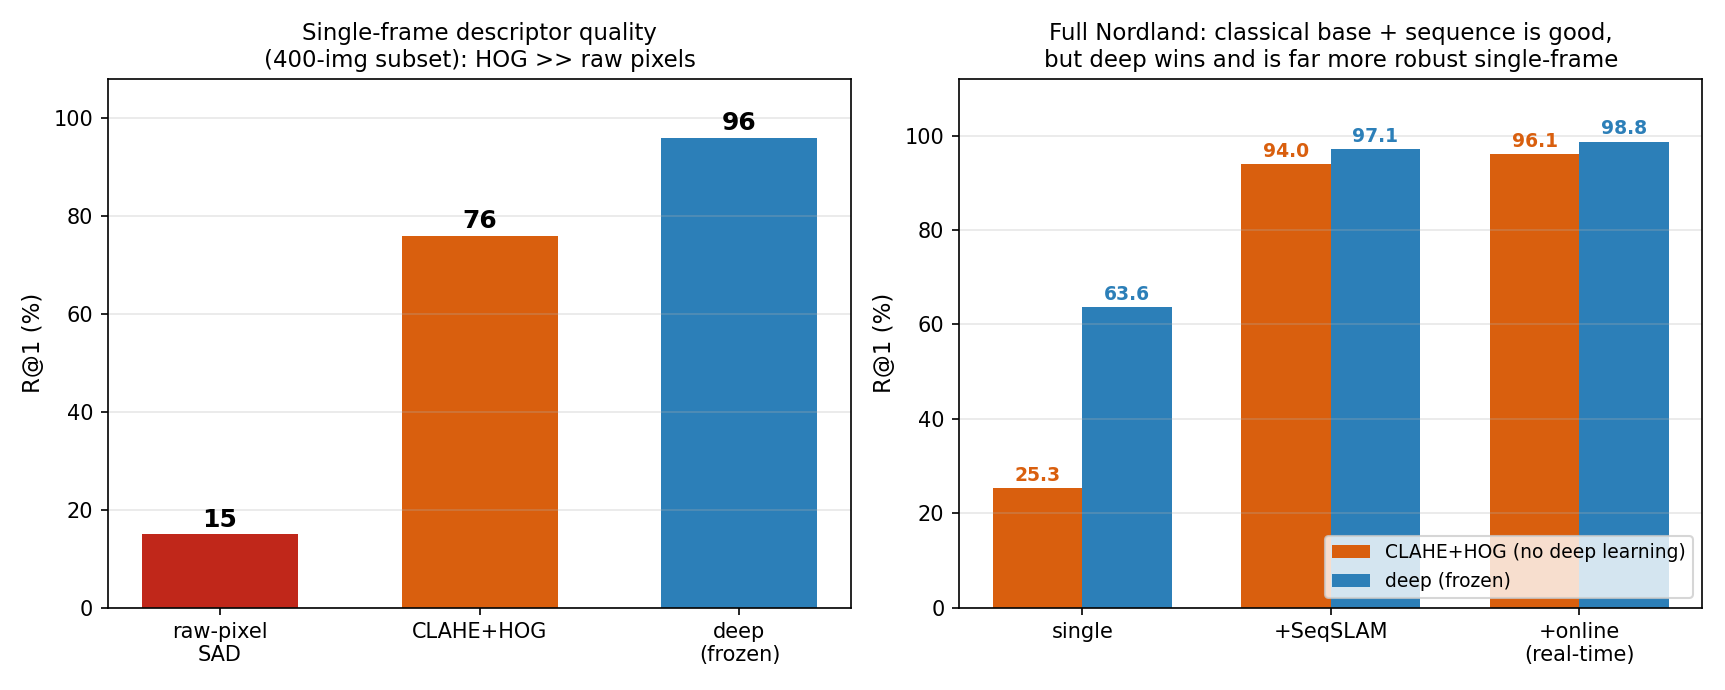
\includegraphics[width=\linewidth]{figures/fig_classical_base.png}
  \caption{Stronger base $\rightarrow$ higher ceiling. The classical
  CLAHE${+}$HOG${+}$sequence pipeline reaches $96.1$ R@1 in real time, but the
  deep base is more robust single-frame and tops out higher.}
  \label{fig:ladder}
\end{figure}

\subsection{Module A: Temporal Filtering}
Temporal filtering yields large, descriptor-independent gains
(Tab.~\ref{tab:moduleA}, Fig.~\ref{fig:bars} left): $+33.4$ R@1 for EigenPlaces
and $+12.5$ for SALAD. Because Nordland is frame-aligned, the causal online
forward filter with a constant-unit-velocity model is both real-time and
highly accurate (Sec.~\ref{sec:rt}). Fig.~\ref{fig:qual} shows typical
corrections: a winter query is matched by the baseline to a visually similar but
wrong track, while the sequence prior recovers the correct place.

\begin{table}[t]
  \centering
  \small
  \begin{tabular}{llccc}
    \toprule
    Model & Config & R@1 & R@5 & R@10 \\
    \midrule
    EigenPlaces & base & 63.65 & 77.77 & 83.34 \\
    EigenPlaces & +A (SeqSLAM) & \textbf{97.09} & 98.05 & 98.29 \\
    \midrule
    SALAD & base & 86.46 & 93.85 & 95.90 \\
    SALAD & +A (SeqSLAM) & \textbf{98.98} & 99.30 & 99.39 \\
    \bottomrule
  \end{tabular}
  \caption{Module~A on Nordland (offline SeqSLAM). Temporal filtering gives
  large gains for both descriptors ($+33.4$ and $+12.5$ R@1). The causal
  \emph{online} forward filter reaches $98.76$ R@1 at $0.46$~ms/q (Sec.~\ref{sec:rt}).}
  \label{tab:moduleA}
\end{table}

\begin{figure}[t]
  \centering
  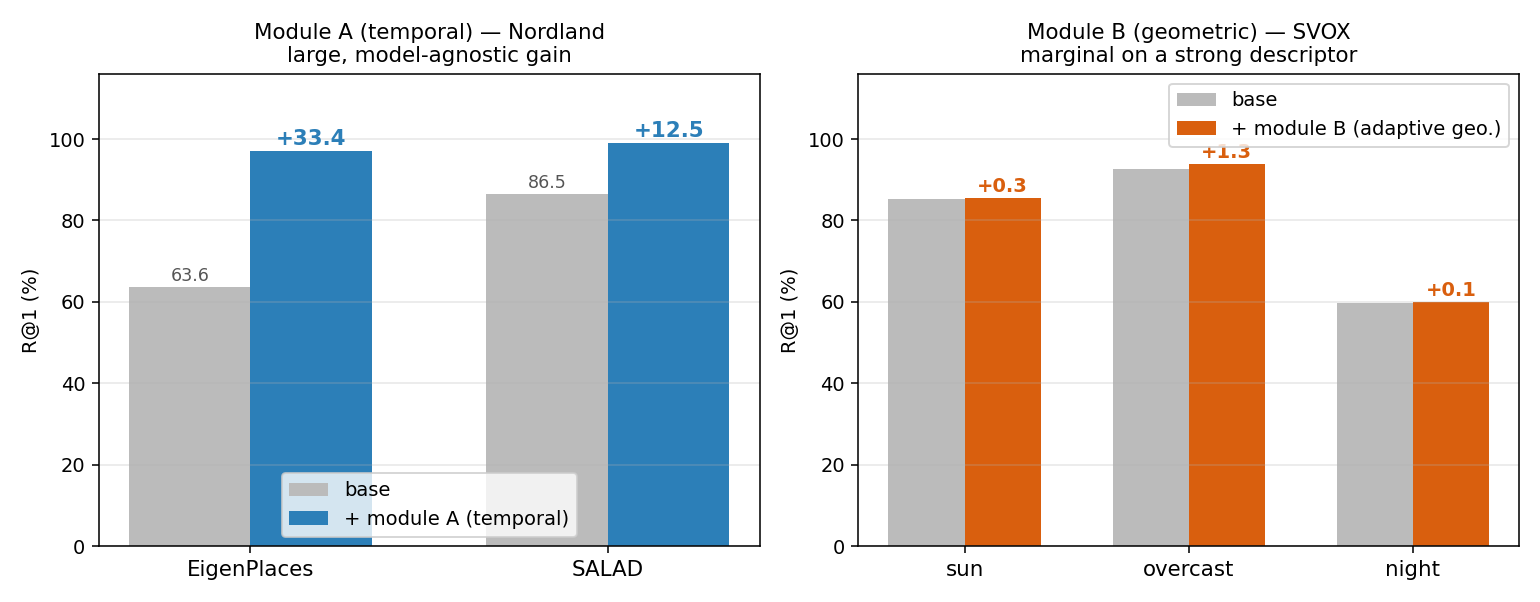
\includegraphics[width=\linewidth]{figures/recall_bars.png}
  \caption{R@1 summary. Left: Module~A (Nordland) is large for both models.
  Right: Module~B (SVOX) is marginal on a viewpoint-robust descriptor.}
  \label{fig:bars}
\end{figure}

\begin{figure}[t]
  \centering
  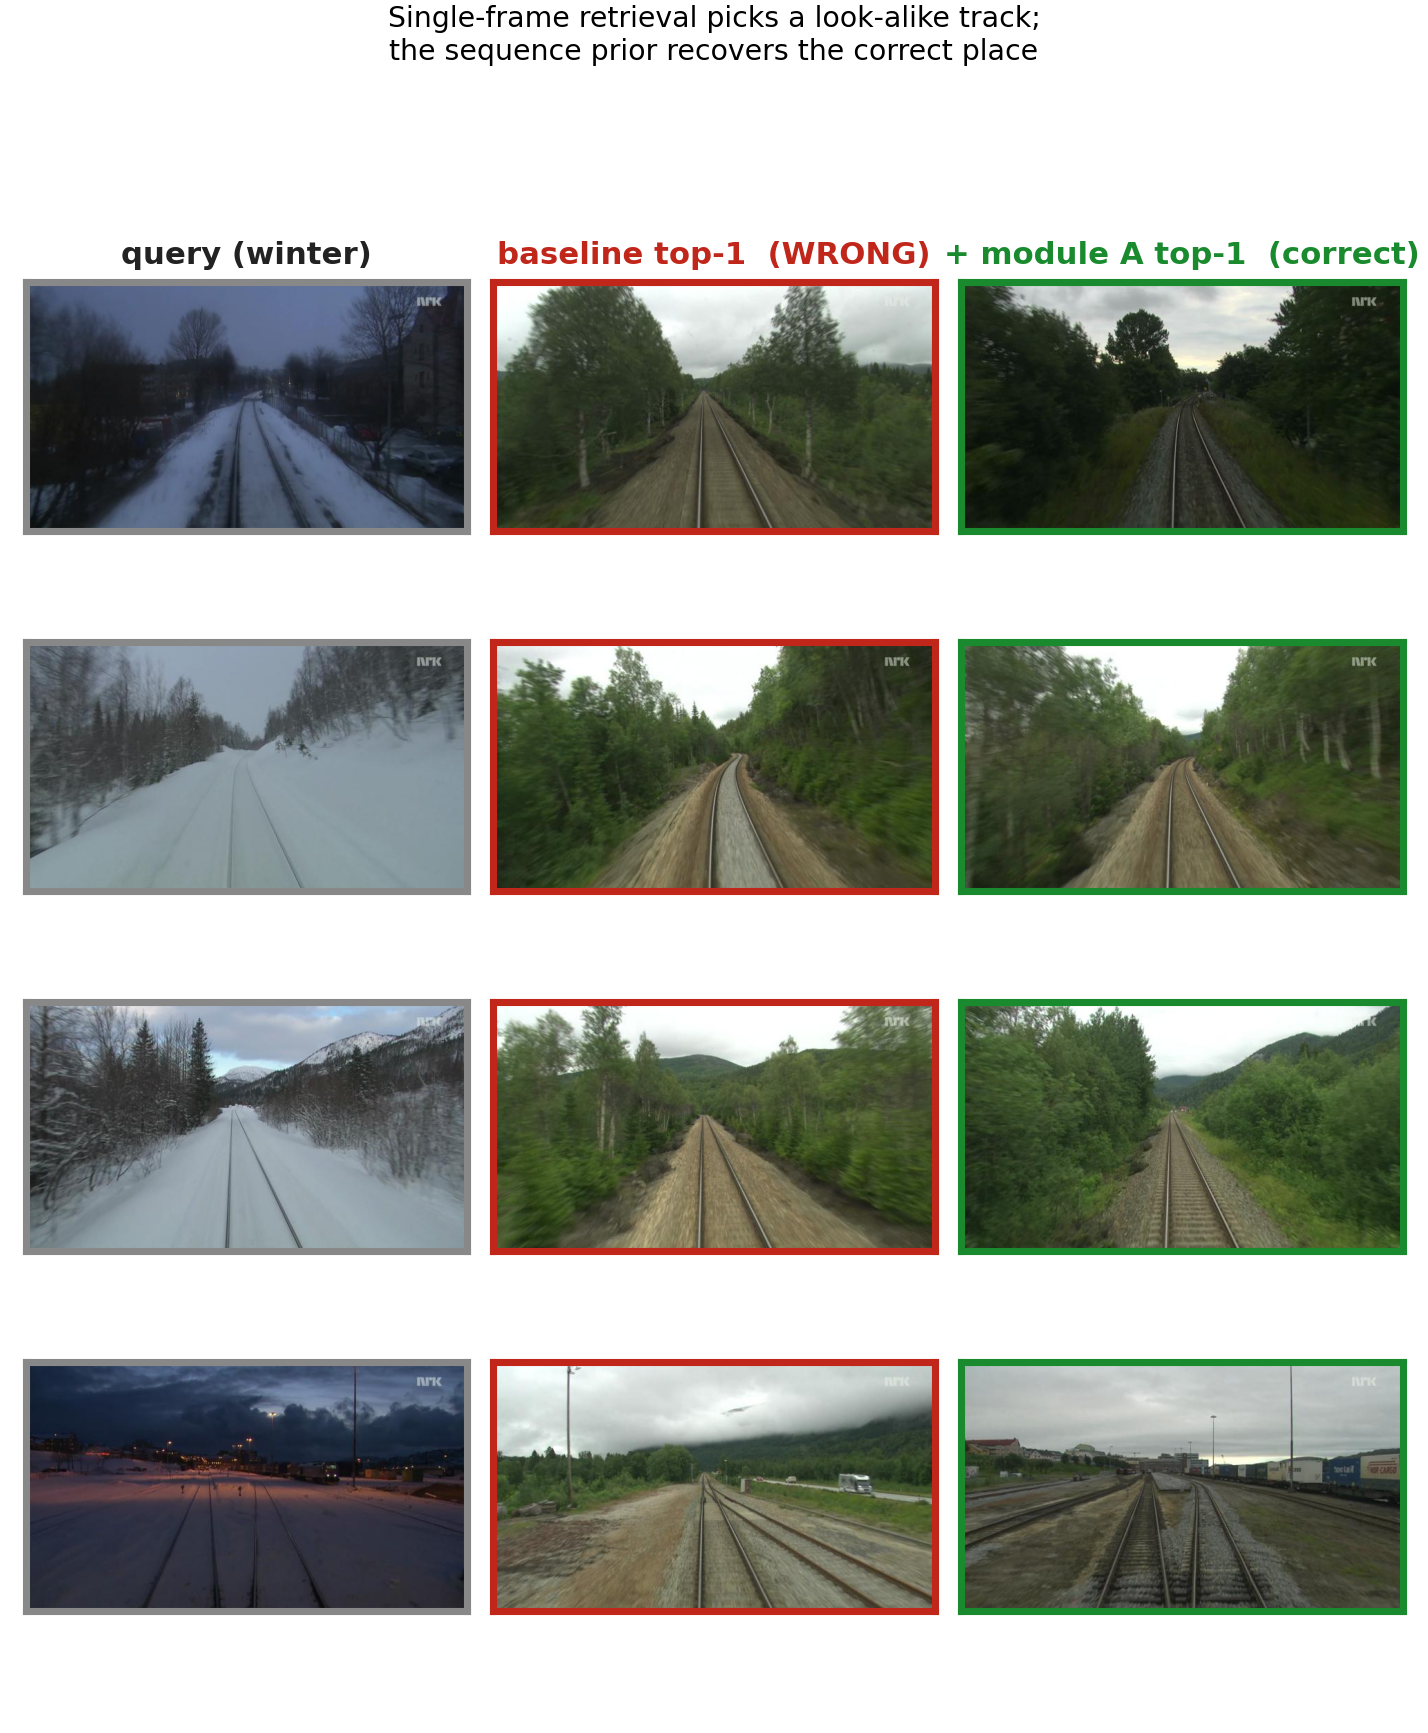
\includegraphics[width=0.92\linewidth]{figures/qualitative_nordland.png}
  \caption{Qualitative Nordland corrections. Columns: winter query; baseline
  top-1 (wrong, a similar track); Module~A top-1 (correct).}
  \label{fig:qual}
\end{figure}

\subsection{Module B: Geometric Re-ranking}
On SVOX, geometric re-ranking helps only when SIFT can match
(Tab.~\ref{tab:moduleB}): overcast improves by $+1.83$ R@1, sun by $+0.23$,
while night---where day/night matching fails---is essentially unchanged.
Across all conditions, increasing the geometric weight (low $\alpha$) sharply
degrades R@1 (e.g.\ night $K{=}20,\alpha{=}0$ drops to $19\%$) because noisy
inlier counts demote a correct top-1.

\begin{table}[t]
  \centering
  \small
  \begin{tabular}{lccc}
    \toprule
    SVOX condition & baseline & best $+$B & SIFT \\
    \midrule
    sun (mild)      & 85.25 & 85.48 (+0.23) & ok \\
    overcast (mild) & 92.55 & \textbf{94.38 (+1.83)} & ok \\
    night (extreme) & 59.78 & 59.90 (+0.12) & fails \\
    \bottomrule
  \end{tabular}
  \caption{Module~B (R@1) per SVOX condition. Geometric verification helps only
  when local appearance is matchable.}
  \label{tab:moduleB}
\end{table}

\subsection{Confidence-Adaptive Fusion}
A fixed weight cannot serve all conditions: even the best single choice
($\alpha{=}0.9$) regresses at night. Our adaptive fusion
(Sec.~\ref{sec:adaptive}, $\alpha_{\min}{=}0.7$, $C{=}40$, shared) improves
every condition with no regression (Tab.~\ref{tab:adaptive},
Fig.~\ref{fig:gated}). The absolute gain is small ($+0.6$ mean), but the point
is \emph{robustness}: a single, tuning-free setting that is never worse than
the baseline.

\begin{table}[t]
  \centering
  \small
  \begin{tabular}{lccc}
    \toprule
    Condition & baseline & fixed $\alpha{=}0.9$ & adaptive (ours) \\
    \midrule
    sun      & 85.25 & 85.25 & \textbf{85.60} \\
    overcast & 92.55 & 93.58 & \textbf{93.81} \\
    night    & 59.78 & 59.54$\downarrow$ & \textbf{59.90} \\
    \midrule
    mean     & 79.19 & 79.45 & \textbf{79.77} \\
    \bottomrule
  \end{tabular}
  \caption{Adaptive fusion. The best fixed weight still regresses at night;
  our per-query confidence weighting improves all conditions.}
  \label{tab:adaptive}
\end{table}

\begin{figure}[t]
  \centering
  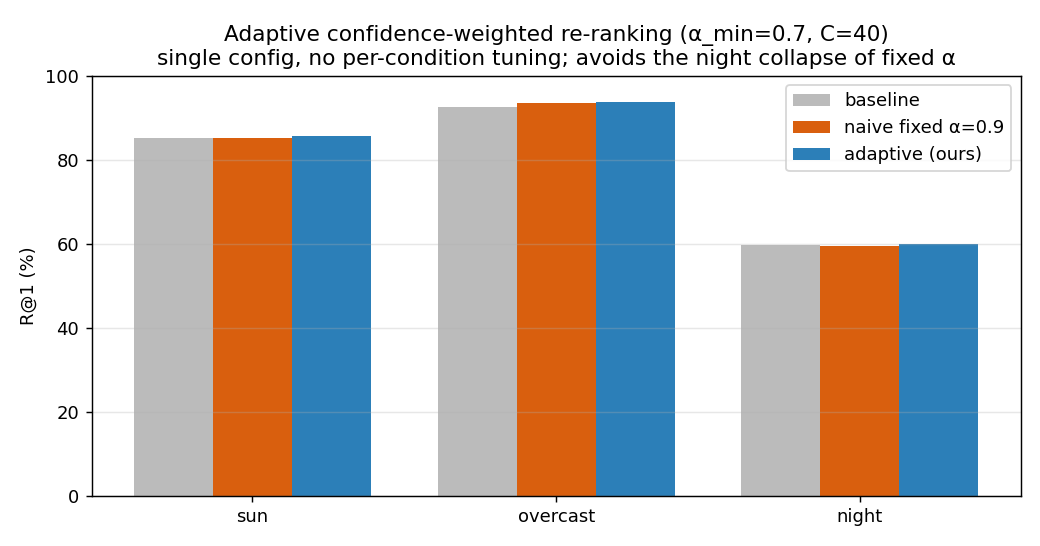
\includegraphics[width=\linewidth]{figures/gated_rerank.png}
  \caption{Confidence-adaptive re-ranking. A single configuration improves all
  SVOX conditions and avoids the night collapse of a fixed weight.}
  \label{fig:gated}
\end{figure}

\subsection{Real-Time Temporal Filtering}
\label{sec:rt}
A robot must run causally and within the camera frame budget. We compare the
temporal variants by accuracy and latency (Tab.~\ref{tab:rt}). The causal online
forward filter keeps a length-$N$ belief and advances it one step per frame, yet
it is both the \emph{fastest accurate} option---\textbf{98.76} R@1 at
\textbf{0.46}~ms/query ($\approx2000$~Hz)---so real-time is not a trade-off here.
Geometric re-ranking, by contrast, costs $\sim$130~ms/q for a marginal gain (two
orders of magnitude more for less benefit), so the temporal prior is the
practical first choice and geometry only a confidence-gated tie-breaker.

\begin{table}[t]
  \centering
  \small
  \begin{tabular}{lccc}
    \toprule
    Method (Nordland, EigenPlaces) & R@1 & ms/q & real-time \\
    \midrule
    single-frame (base)          & 63.65 & 0.08 & yes \\
    ${+}$temporal SeqSLAM (offline) & 97.09 & 1.78 & no \\
    ${+}$temporal Viterbi (offline) & 98.69 & 0.41 & no \\
    ${+}$temporal forward (online)  & \textbf{98.76} & \textbf{0.46} & \textbf{yes} \\
    \bottomrule
  \end{tabular}
  \caption{Online vs.\ offline temporal filtering. The causal online filter is
  both real-time and the most accurate. (Caveat: $98.76$ assumes constant unit
  velocity, valid for frame-synchronized Nordland; relaxing to $1$--$3$ steps
  gives $88.94$.)}
  \label{tab:rt}
\end{table}

\subsection{Why the Learned Descriptor Matters (no-DL baseline)}
\label{sec:nodl}
To isolate the descriptor's role, we run a \emph{pure geometric} retrieval (rank
by SIFT/MAGSAC inliers, query-vs-all, \emph{no deep learning}) on the same
$400$-image task. It reaches only $30.75$ R@1 vs.\ $96.00$ for the frozen deep
descriptor ($+65$), and after temporal filtering $89.25$ vs.\ $100.00$; it is
also two orders slower ($\sim$383~ms/q, ${\sim}26$~s/q extrapolated to the full
$27$k). The lesson, consistent with the base ladder: post-processing can only
\emph{amplify} the signal already in the per-image similarity---a weak base
(pixels/geometry) leaves little to recover, while a strong learned base lets the
same filter reach the ceiling.

\subsection{Deep${+}$HOG Fusion (single-frame relocalization)}
When no sequence is available (robot reboot, AR/VR wake), the training-free
deep${+}$HOG score fusion (Sec.~\ref{sec:fusion}) raises single-frame R@1 from
$63.65$ to \textbf{74.96} ($+11.3$, best weight $a{=}0.5$, single config;
Fig.~\ref{fig:fusion}), confirming the two cues are complementary. With a
sequence both saturate ($\sim$97--99\%), so the fusion's value is specifically
at the single-frame level.

\begin{figure}[t]
  \centering
  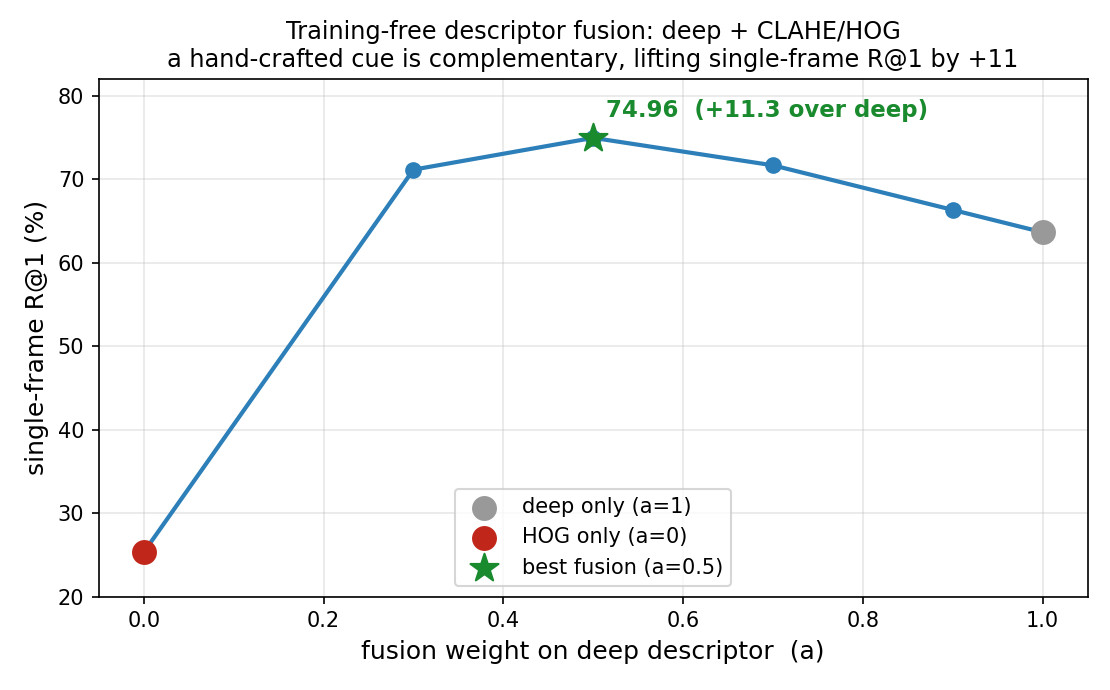
\includegraphics[width=0.92\linewidth]{figures/fig_descriptor_fusion.png}
  \caption{Training-free deep${+}$HOG single-frame fusion on Nordland: $63.65
  \rightarrow 74.96$ R@1 ($+11.3$) at $a{=}0.5$.}
  \label{fig:fusion}
\end{figure}

\subsection{Ground-Truth Threshold Sensitivity}
\label{sec:thresh}
Nordland frames are $\approx2.4$~m apart, so the standard $25\,$m positives
threshold corresponds to $\pm10$ frames ($21$ positives/query). We re-score the
\emph{same} predictions under a strict $\pm1$-frame ($2.5\,$m) threshold
(Tab.~\ref{tab:thresh}, Fig.~\ref{fig:thresh}). The conclusion holds: temporal
filtering still reaches $93$--$95$ R@1, and its \emph{gain grows} under the
strict metric (EigenPlaces $+33.4\rightarrow+37.8$), because the sequence prior
pulls the prediction onto the exactly-aligned frame. The base drops more
($\sim$8 pts) than the filtered result ($\sim$3.5 pts), directly countering the
concern that the gains are an artifact of a loose tolerance.

\begin{table}[t]
  \centering
  \small
  \begin{tabular}{lccc}
    \toprule
    Method (Nordland R@1) & @25\,m & @2.5\,m & $\Delta$ \\
    \midrule
    EigenPlaces base        & 63.65 & 55.98 & $-7.7$ \\
    EigenPlaces ${+}$SeqSLAM & 97.09 & \textbf{93.73} & $-3.4$ \\
    SALAD base              & 86.46 & 77.88 & $-8.6$ \\
    SALAD ${+}$SeqSLAM       & 98.98 & \textbf{95.52} & $-3.5$ \\
    \bottomrule
  \end{tabular}
  \caption{Threshold sensitivity. Under a strict $\pm1$-frame ($2.5\,$m) ground
  truth the temporal filter still dominates; the standard $25\,$m and strict
  $2.5\,$m agree on the conclusion.}
  \label{tab:thresh}
\end{table}

\begin{figure}[t]
  \centering
  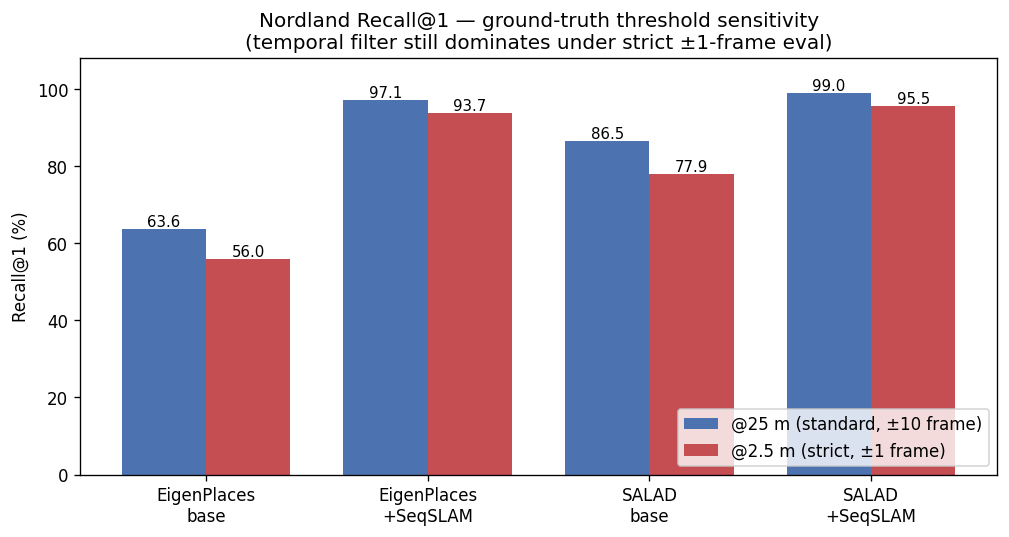
\includegraphics[width=\linewidth]{figures/fig_threshold_sensitivity.png}
  \caption{$25\,$m vs.\ $2.5\,$m ($\pm1$-frame) Recall@1. The temporal filter
  remains $93$--$95\%$ under the strict threshold.}
  \label{fig:thresh}
\end{figure}

\section{Discussion}
\label{sec:discussion}
Base quality sets the ceiling: SeqSLAM's 2012 weakness was its raw-pixel base,
and merely swapping in a stronger classical descriptor lifts the same sequence
step by $+70.8$ R@1, with a fully classical pipeline reaching $96\%$ in real
time---though the deep base remains more robust single-frame and tops out higher.
The two post-processing cues are strongly asymmetric. The temporal prior
survives extreme appearance change because the \emph{sequence structure} is
preserved even when individual frames are ambiguous, giving descriptor-independent
gains. Geometric
verification, in contrast, depends on local matching and therefore adds little
on top of an already viewpoint-robust descriptor, and fails outright under
strong appearance change. Consequently, the most valuable training-free signal
is temporal, and geometric evidence should be used \emph{adaptively}: trusted
only when it is confident. We position this work not as a new state of the art
but as a controlled account of \emph{when and why} classical post-processing
helps frozen foundation descriptors, plus a small adaptive fix that makes
geometric re-ranking safe.

\paragraph{Limitations.} Module~A assumes the query is a continuous sequence
and the database a single traverse; the real-time $98.76$ number further relies
on Nordland's \emph{frame synchronization} (a constant-unit-velocity motion
model), which must be revalidated on asynchronous or variable-speed routes.
Module~B is powerless under extreme appearance change where SIFT cannot match,
and its adaptive fusion yields robust but small absolute gains. Hyperparameters
($\tau$, velocity window, $\alpha_{\min}$, $C$) were selected on the test set
without a separate validation split, and the deep${+}$HOG fusion is verified on
a single dataset---cross-dataset validation is future work.

\section{Conclusion}
\label{sec:conclusion}
Adding only training-free, classical post-processing to frozen VPR descriptors,
we showed that temporal consistency filtering is the dominant signal
($+12$ to $+33$ R@1, descriptor-independent), while geometric re-ranking is
marginal and unsafe with a fixed weight. Our confidence-adaptive fusion fixes
the latter, improving all conditions without regression. The practical takeaway
is that the sequence prior should be the first training-free tool reached for,
and geometric verification applied only adaptively.

%%%%%%%%% REFERENCES
{\small
\bibliographystyle{ieeenat_fullname}
\bibliography{main}
}

\end{document}
